%-----------------------------------------------------------------------------%
 \chapter{\babSatu}
%-----------------------------------------------------------------------------%
%-----------------------------------------------------------------------------%
\section{Latar Belakang Masalah}
%-----------------------------------------------------------------------------%\todo{Ceritakan latar belakang penelitian ini.}
\begin{figure}[b!]
	\centering
	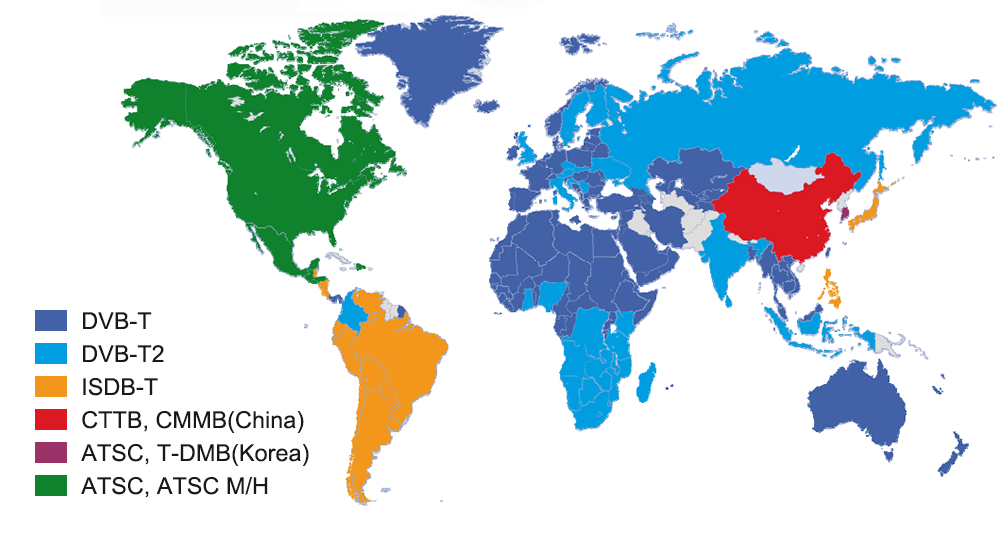
\includegraphics[width=1\textwidth]
		{pics/standar.png}
		\caption{Klasifikasi standar TV digital dunia.}
	\label{fig:Klasifikasi Standar TV Digital Dunia}
\end{figure}
Indonesia telah melakukan migrasi dari penyiaran televisi (TV) analog ke TV digital dengan menggunakan standar \textit{Digital Video Broadcasting-Terrestrial} \text{(DVB-T)} sejak tahun 2007 \cite{regul2}. Saat ini, perkembangan TV \text{digital} di dunia sangat pesat. Berbagai negara telah menggunakan standar \text{\textit{Digital Video Broadcasting - Second Generation Terrestrial}} (DVB-T2) menggantikan standar DVB-T dikarenakan DVB-T2 menggunakan besar spektrum yang sama, tetapi dapat mengirimkan lebih banyak program siaran TV atau dapat mengirimkan kualitas video/audio yang lebih baik daripada DVB-T \cite{itu}. Indonesia diharapkan di masa mendatang dapat melakukan transisi dari DVB-T ke DVB-T2 secara menyeluruh, sesuai dengan regulasi dari Menteri Komunikasi dan Infomatika (Menkominfo) DVB-T2 akan menggantikan standar DVB-T di Indonesia \cite{regul}.

Transisi dari DVB-T ke \text{DVB-T2} memerlukan banyak persiapan. Untuk memperoleh kinerja optimal standar DVB-T2 harus disesuaikan dengan kondisi alam (\textit{channel model}) Indonesia. DVB-T2 menggunakan \textit{Low Density Parity Check} (LDPC) \textit{codes} sebagai \textit{channel coding} di \textit{inner coding} dari \textit{Frame Error Correction} (FEC) \cite{etsi1}. Untuk melakukan migrasi dari DVB-T ke DVB-T2 di Indonesia struktur dan \textit{code rate} LDPC \textit{codes} DVB-T2 yang sesuai dengan \textit{channel model} \text{Indonesia} diperlukan. Penyesuaian LDPC \textit{codes} DVB-T2 diperlukan agar LDPC \textit{codes} dapat bekerja secara optimal, sehingga memiliki peluang \textit{error} menjadi sangat kecil. 

Tantangan utama untuk melakukan transisi dari DVB-T ke DVB-T2 adalah standar DVB-T2 yang diterbitkan oleh \textit{European Telecommunications Standards Institute} (ETSI), merupakan standar untuk menerapkan DVB-T2 di Jerman \cite{etsi2}. Indonesia memiliki \textit{channel model} yang sangat berbeda dari Jerman, oleh karena itu diperlukan standar DVB-T2 yang sesuai dengan \textit{channel model} di Indonesia sehingga DVB-T2 dapat memperoleh kinerja yang optimal. Tugas Akhir ini bertujuan memperoleh standar FEC di bagian \textit{inner coding} dari DVB-T2 yang sesuai dengan \textit{channel model} Indonesia untuk penerapan DVB-T2 di Indonesia kedepannya.   

Hasil yang diharapkan dari Tugas Akhir ini adalah struktur dan \textit{code rate} optimal dari LDPC \textit{codes} DVB-T2 yang sesuai dengan \textit{channel model} \text{Indonesia}. Pengujian kinerja menggunakan metode \textit{Extrinsic Information Transfer} (EXIT) \textit{chart} serta simulasi pada kanal \text{\textit{Additive White Gaussian Noise}} (AWGN) dan \textit{frequency-selective} \textit{fading} menggunakan aplikasi MATLAB, hasil divalidasi \text{dengan} teori dasar, sehingga hasil kinerja \textit{inner coding} dari FEC DVB-T2 ini optimal. 

%-----------------------------------------------------------------------------%
\section{Rumusan Masalah}
%-----------------------------------------------------------------------------%
Sejak tahun 2012 Menkominfo telah menetapkan DVB-T2 sebagai standar penyiaran TV digital di Indonesia \cite{regul}, tapi sampai saat ini Indonesia belum memiliki standar spesifikasi DVB-T2 yang sesuai dengan \textit{channel model} Indonesia. Salah satu spesifikasi DVB-T2 adalah \textit{inner coding} dari FEC DVB-T2 yaitu LDPC \textit{codes}. Tidak adanya struktur optimal ini menyebabkan tidak diketahuinya karakteristik kinerja DVB-T2 Indonesia yang menyebabkan sulitnya industri membuat produk yang terbaik dan sesuai standar Indonesia.

%-----------------------------------------------------------------------------%
\section{Tujuan Penelitian}

Tugas Akhir ini bertujuan melakukan studi pada struktur dan nilai \textit{code rate} LDPC \textit{codes} DVB-T2 yang dievaluasi dengan \textit{channel model} Indonesia, sehingga kinerja TV digital Indonesia bisa diketahui. Hasil ini bermanfaat juga bagi industri dalam mengembangkan alat-alat pemancar dan penerima TV digital.


%-----------------------------------------------------------------------------%
\section{Batasan Masalah}
Tugas Akhir ini memiliki batasan masalah sebagai berikut:
\begin{enumerate}
	\item Menguji kinerja LDPC \textit{codes} DVB-T2 menggunakan \textit{code rate} $\frac{1}{2}, \frac{3}{5}, \frac{2}{3}, \frac{3}{4}, \frac{4}{5},$ dan $\frac{5}{6}$ pada DVB-T2 LDPC \textit{codes} dengan panjang blok $N_{LDPC}=16200$.
	\item Simulasi menggunakan kanal AWGN dan \textit{frequency selective fading} pada \textit{channel model} DVB-T2 di Indonesia.
	\item Untuk simplifikasi penelitian, maka penulis menggunakan modulasi \textit{Quadrature Phase Shift Keying} (QPSK).     	 
\end{enumerate}
%
%Agar penelitian ini dapat memiliki kualitas baik, Tugas Akhir ini membatasi pokok bahasan hanya pada LDPC \textit{codes} yang sesuai dengan standar DVB-T2. Tugas Akhir ini menganalisis kinerja LDPC \textit{codes} menggunakan analisis EXIT \textit{chart}, lalu mensimulasikan kinerja \textit{codes} menggunakan AWGN dan \textit{frequency-selective fading channel}. Apabila tidak ada LDPC \textit{codes} yang optimal dari standar DVB-T2, maka Tugas Akhir ini akan memodifikasi LDPC \textit{codes} dari DVB-T2 agar memiliki kinerja optimal untuk Indonesia.           
%
%Untuk menghindari pembahasan yang terlalu luas, Proposal Tugas Akhir ini hanya akan membahas, diantaranya :
%\begin{itemize}
%	\item[a.]Nilai \textit{rate} dari LDPC \textit{code} yang cocok dengan kanal Indonesia.
%	\item[b.]Merancang LDPC \textit{code} DVB-T2 yang sesuai dengan kanal Indonesia. 
%	\item[c.]Nilai BER, BLER, \textit{outage probability} dari LDPC \textit{code} DVB-T2 yang sesuai dengan kanal Indonesia. 
%\end{itemize}

\section{Metodologi Penelitian}
Tugas Akhir ini menerapkan metodologi penelitian sebagai berikut:	
\begin{itemize}
	\item[a.] Studi Literatur\\	
	Tahap ini melakukan pengumpulan informasi, menganalisis, dan mengidentifikasi tentang LDPC \textit{codes} secara umum dan LDPC \textit{codes} DVB-T2 dari berbagai literatur. Literatur yang menjadi rujukan adalah \textit{text book}, \textit{thesis}, buku disertasi, standar DVB-T2, dan jurnal atau \textit{paper conference} internasional yang dipublikasikan \textit{Institute of Electrical and Electronics Engineers} (IEEE).
	\item[b.] Simulasi pada Kanal AWGN dan \textit{Frequency Selective} \textit{Fading}\\
	Tahap ini bertujuan untuk mengevaluasi kinerja LDPC \textit{codes} DVB-T2 pada kanal AWGN dan \textit{channel model} DVB-T2 Indonesia.
	\item[c.] Perancangan Struktur\\	
	Tahap ini melakukan perancangan struktur LDPC \textit{codes} berdasarkan hasil yang didapat pada tahap (b), jika hasil sudah sesuai, maka perancangan struktur \textit{code} yang baru menjadi minimal. Apabila hasil kurang bagus, maka perancangan struktur akan cukup banyak. 
%	melakukan simulasi menggunakan aplikasi komputer Matlab dari LDPC \textit{codes} DVB-T2 dengan menggunakan \textit{code rate} yang tersedia di standar DVB-T2 pada AWGN dan frekuensi selektif \textit{fading channel}, lalu dioptimalisasi menggunakan EXIT \textit{chart}.
	\item[d.] Analisis EXIT \textit{Chart}\\
	Tahap ini menganalisis struktur dan \textit{code rate} dari LDPC \textit{codes} DVB-T2 untuk menghasilkan kurva EXIT \textit{chart} yang tidak berpotongan  untuk mengetahui kinerja yang paling baik.  
	\item[e.] Studi Analisis\\
	Tahap ini menganalisis hasil simulasi dari semua \textit{code rate} LDPC \textit{codes} DVB-T2 pada tahap sebelumnya. Analisis dilakukan terhadap EXIT \textit{chart}, \textit{girth}, dan kinerja \textit{Bit Error Rate} (BER) pada kanal AWGN dan \textit{frequency-selective fading} menggunakan \textit{channel model} DVB-T2 Indonesia
%	AWGN dan frekuensi selektif \textit{fading channel} yang dibandingkan dengan \textit{shannon-limit} serta dievaluasi menggunakan metode EXIT \textit{chart}. Apabila tidak ditemukan struktur dan \textit{code rate} yang memiliki kinerja optimal dengan parameter gap \textit{shannon-limit} kurang dari 1 dB dan kurva dari EXIT chart tidak saling  berpotongan, 
	\item[f.] Penarikan Kesimpulan\\
	Tahap ini menarik kesimpulan dari seluruh hasil evaluasi dan usulan untuk LDPC \textit{codes} pada DVB-T2.  
\end{itemize}

%\section{Jadwal Pelaksanaan}
%%-----------------------------------------------------------------------------%
%Rencana jadwal penelitan Tugas Akhir ini adalah sebagai berikut: \\
%\begin{table}
%\centering
%\caption{Jadwal penelitian}
%
%	\begin{tabular}{| c | L{4cm} | L{1.8cm} | L{3cm} | L{3.5cm} |}
%		\hline
%		\thead{No.} & \thead{Deskripsi Tahapan} & \thead{Durasi} & \thead{Tanggal Selesai} & \thead{\textit{Milestone}}\\
%		\hline
%		1 & Studi struktur LDPC \textit{codes} & 2 minggu & 20-5-2019 & Perbedaan LDPC \textit{codes} umum dan LDPC \textit{codes} DVB-T2 didapat.\\
%		\hline
%		2 & Simulasi pada AWGN \textit{channel} dan \textit{frequency selective fading channel} & 3 minggu & 10-6-2019 & Gap kurang dari 1~dB dengan \textit{Shannon-Limit}.\\
%		\hline
%		3 & Perancangan struktur & 4 minggu & 8-7-2019 & Struktur LDPC \textit{codes} DVB-T2.\\
%		\hline
%		4 & Analisis EXIT \textit{chart} & 3 minggu & 29-7-2019 & Gap terkecil dan tidak saling berpotongan. \\
%		\hline
%		5 & Analisis & 6 minggu & 9-9-2019 & Menentukan perlunya modifikasi dan melakukan modifikasi.\\
%		\hline
%		6 & Penyusunan buku TA & 2 minggu & 23-9-2019 & Buku TA selesai.\\
%		\hline
%%		5 & Analisis performansi & 3 minggu & 2 Juli 2019 & Menganalisis hasil simulasi yang telah dilakukan\\
%%		\hline
%%		6 & Evaluasi simulasi pertama & 3 minggu & 23 Juli 2019 & Mengevaluasi hasil yang telah dianalisis pada tahapan sebelumnya\\
%%		\hline
%%		7 & Simulasi model kedua & 2 bulan & 23 September 2019 & Perancangan dan simulasi BER, BLER, dan \textit{outage probability} dari hasil evaluasi pertama\\
%%	\hline		
%%		8 & Analisis performansi kedua & 3 minggu & 14 Oktober 2019 & Menganalisis hasil simulasi kedua yang telah dilakukan\\
%%		\hline
%%9 & Evaluasi simulasi & 3 minggu & 4 November 2019 & Mengevaluasi hasil analisis performansi kedua\\
%%	\hline
%%10 & Pengajuan \textit{paper} & 4 minggu & 4 Desember 2019 & Menyusun dan menyelesaikan \textit{paper}\\
%%\hline
%%11 & Penyusunan laporan/buku TA & 3 minggu & 28 Desember 2019 & Buku TA selesai\\
%%\hline
%	\end{tabular}
%	
%\end{table}
\section{Sistematika Penulisan}
%-----------------------------------------------------------------------------%
Untuk selanjutnya, Tugas Akhir ini ditulis dengan sistematika sebagai berikut:
\begin{itemize}
%	\item Bab 1 \babSatu \\
%	Bab ini berisi latar belakang, permasalahan, tujuan, metode penelitian, dan sistematika penulisan dari Tugas Akhir.
	\item BAB II \babDua \\
	Bab ini menjelaskan teori dan dasar LDPC \textit{codes}, DVB-T2, dan pendukung penelitian Tugas Akhir ini.
	\item BAB III \babTiga \\
	Bab ini menjelaskan model sistem mulai dari \textit{transmitter}, model kanal, hingga \textit{receiver}, dan posisi LDPC \textit{codes} dalam sistem tersebut. Bab ini juga menjelaskan LDPC \textit{codes} yang diusulkan.	
	\item BAB IV \babEmpat \\
	Bab ini menganalisis dan mengevaluasi kinerja LDPC \textit{codes} DVB-T2 pada kanal AWGN dan \textit{channel model} DVB-T2 Indonesia yang divalidasi dengan parameter praktis BER.
	\item BAB V \babLima \\
	Bab ini berisi kesimpulan hasil studi kinerja LDPC \textit{codes} DVB-T2 dan saran untuk pengembangan lebih lanjut Tugas Akhir ini pada masa mendatang.
\end{itemize}
%\section{Rumusan}
%Ini lhooo
%\begin{itemize}
%\item [1.] apa kah ini \ref{rumus}?
%\item [2.] ini apa ?
%\end{itemize}
%\subsection{Masalah}
%\cite{buku1}
%\begin{figure}
%\centering
%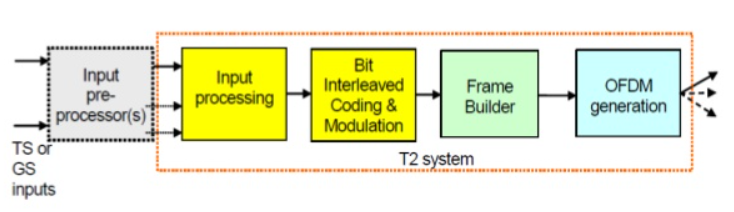
\includegraphics[scale=0.5]{pics/saaa}
%\caption{layer}
%\label {Gambar 1.1: layer}
%\begin{equation}
%\sum_{0}^{100}=\int_{X}^{Y}\cdot\vartheta
%\end{equation}
%\begin{eqnarray}
%\sum_{0}^{100}&=&\int_{X}^{Y}\cdot\vartheta\\
%\sum_{0}^{100}&=&\vartheta
%\label{rumus}
%\end{eqnarray}
%\end{figure}
%\begin{table}
%\begin{center}
%\caption{Perubahan panjang bahan antena}
%\label{tabel: table_tebal}
%\begin{tabular}{|c|c|}
%\hline
%\cellcolor{cyan}Ketebalan bahan & Nilai\\
%\hline
%0.3 cm & -10.64 db\\
%\hline
%\multicolumn{2}{|c|}{0.2cm}\\
%\hline
%0.7 cm & -9.06 db \\
%\hline
%0.1 cm & \multirow{2}{*}{coba}\\
%\cline{1-1}
%0.5 cm & \\
%\hline
%
%
%
%\end{tabular}
%\end{center}
%\end{table}


